\section{Conclusões}

A prática permitiu compreender e distinguir o comparador simples do comparador com histerese, bem como ajudou a compreender o funcionamento na prática desses circuitos, permitindo entender as limitações impostas. 

A prática se mostrou um desafio em quesitos de precisão para encontrar os valores de transição e \textit{offset}, pois o ajuste do potenciômetro deveria ser cuidadoso, porém a modificação do circuito divisor de tensão de forma a permitir que a tensão $V_{in}$ assumisse uma faixa menor de valores contribuiu para que o ajuste fosse realizado de forma mais precisa.

Dessa forma, mesmo com as dificuldades encontradas, permitiu-se encontrar uma ótima correspondência entre os valores teóricos com os práticos, implicando que os circuitos propostos de fato possuem um valor prático de aplicação.

%\newpage

\section{Anexos}

\begin{figure}[H] 
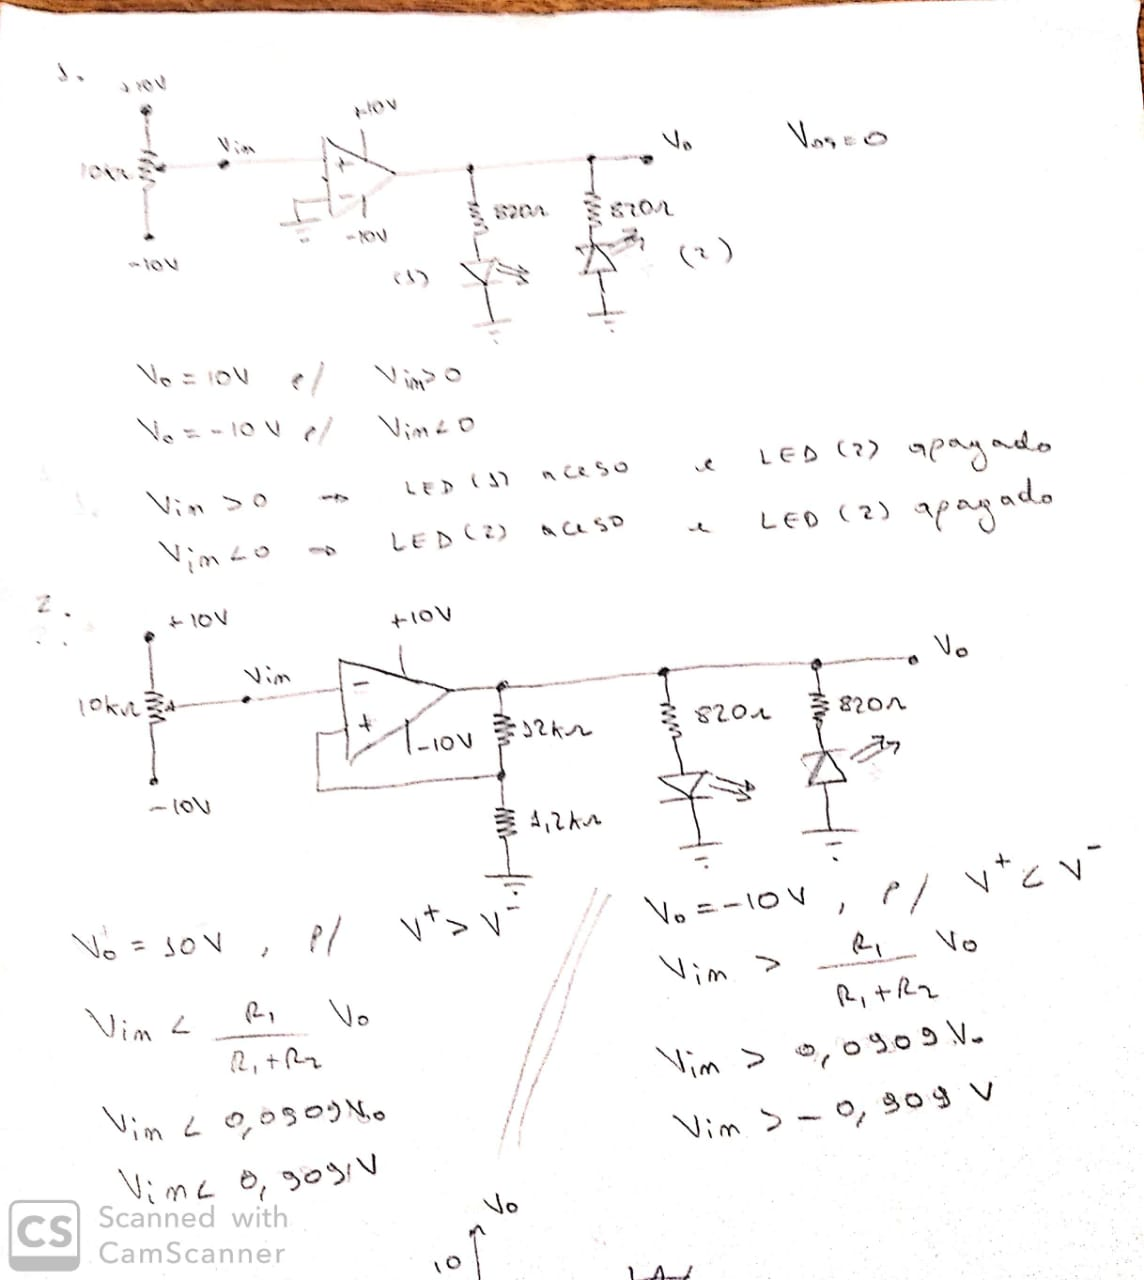
\includegraphics[scale=0.4]{images/calc.jpeg} 
\centering
\caption{Folha de cálculos da prática.}
\label{p5-2} 
\end{figure} 

